\documentclass{article}

\usepackage{color}
\usepackage{graphicx}
\usepackage{amsmath}
\usepackage{bm}
\usepackage{enumerate}
\usepackage{booktabs}
\usepackage{cite}
\usepackage{geometry}
\usepackage{url}
\usepackage{float}
\usepackage{indentfirst}
\usepackage{ulem}
\usepackage{multirow}
\begin{document}

\vspace*{0.25cm}

\hrulefill

\thispagestyle{empty}

\begin{center}
\begin{large}
\sc{UM--SJTU Joint Institute \vspace{0.3em} \\ Introduction to Circuits \\(Ve215)}
\end{large}

\hrulefill

\vspace*{5cm}
\begin{Large}
\sc{{Laboratory Report}}
\end{Large}

\vspace{2em}

\begin{large}
\sc{{Lab 2
\vspace{0.5em}

Op Amp Lab}}
\end{large}
\end{center}
\vfill

\begin{table}[h!]
\centering
\begin{tabular}{ll}
Name: Kang Jiaming \hspace*{2em}&
ID: 518021911220\hspace*{2em}\\

\\

Date:  2019.10.25

\end{tabular}
\end{table}

\hfill
\newpage



		\section{Introduction\label{intro}}
	\subsection{Objectives}
\noindent The goals for this lab are:
\begin{enumerate}
\item Learn how to build and test a variety of circuits based on LM 741 Op Amp chip: non-inverting and inverting amplifiers with fixed gain. 
\item Measure the gain of the amplifier and compare it with theoretical calculations.
\item Determine the saturated output voltage of the amplifier.  
\end{enumerate}

	\subsection{Apparatus and Theoretical Background}
\subsubsection{Op Amp terminals}
\begin{figure}[H]
\centering
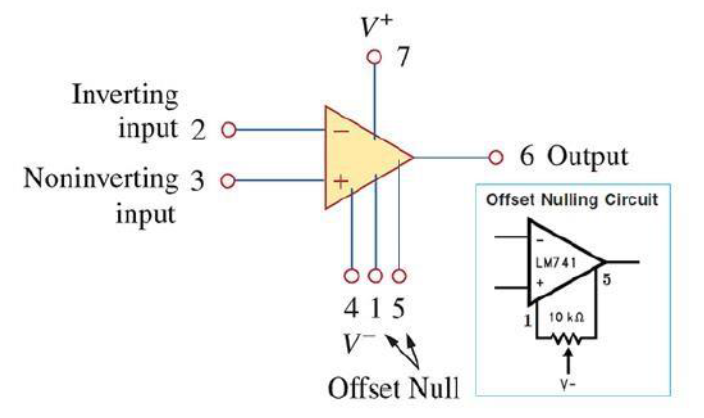
\includegraphics[scale=1.0]{opamp.png}
\caption{Circuit symbol of a typical op amp.}\label{FigOpAmp}
\end{figure}

In Figure \ref{FigOpAmp}, there are:
\begin{enumerate}
\item Two terminals for input signs: inverting (labeled -) and non-inverting (labeled +)
\item A terminal for the output signal
\item Two terminals for the power supply voltages: positive +Vcc and negative -Vcc. (e.g. In this lab, set +Vcc = 5V; -Vcc = -5V.)
\end{enumerate}

Accordingly, for LM741 op amp chip you see in reality, the pin numbers are shown in Figure \ref{FigPin}.

\begin{figure}[H]
\centering
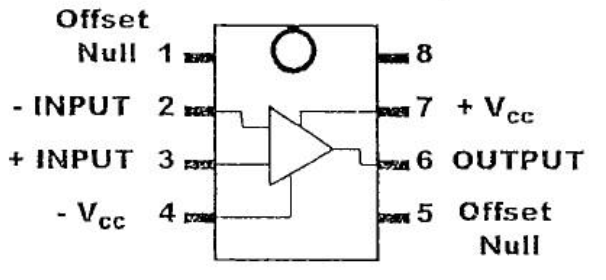
\includegraphics[scale=1]{pin.png}
\caption{Pin numbers for LM 741 op amp.}\label{FigPin}
\end{figure}
\begin{enumerate}
\item Pin $\sharp$8 is not connected; pins $\sharp$1 and $\sharp$5 are not used in this lab.
\item Do not mistake the connections of input signals ($\sharp$2 labeled – and $\sharp$3 labeled +) for the connections to the power supply ($\sharp$4 for -Vcc and $\sharp$7 for +Vcc).
\item Make sure you connect the grounds of oscilloscope, function generator and DC source together.
\end{enumerate}

\subsubsection{The gain of amplifier circuits}

The amplifier circuits are characterized by their gain values. The voltage gain is the ratio of output voltage to the input voltage in the circuit: 
$$Voltage\,\,Gain = \frac{Output\,\,Voltage}{Input\,\,Voltage}$$

\subsubsection{Inverting amplifier}

\begin{figure}[H]
\centering
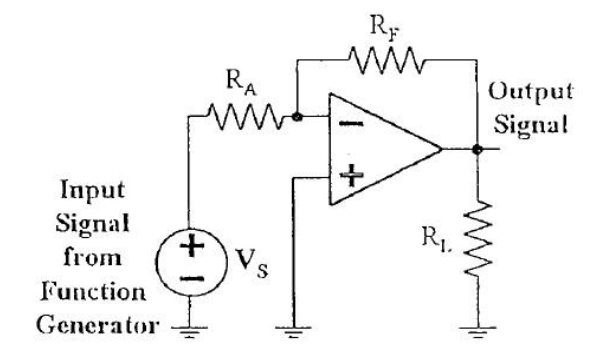
\includegraphics[scale=1]{inverting.png}
\caption{Inverting amplifier.}\label{FigInv}
\end{figure}

For inverting amplifier, the theoretical gain should be:
$$Gain = \frac{V_{output}}{V_S} = -\frac{R_F}{R_A}$$

\subsubsection{Non-inverting amplifier}

\begin{figure}[H]
\centering
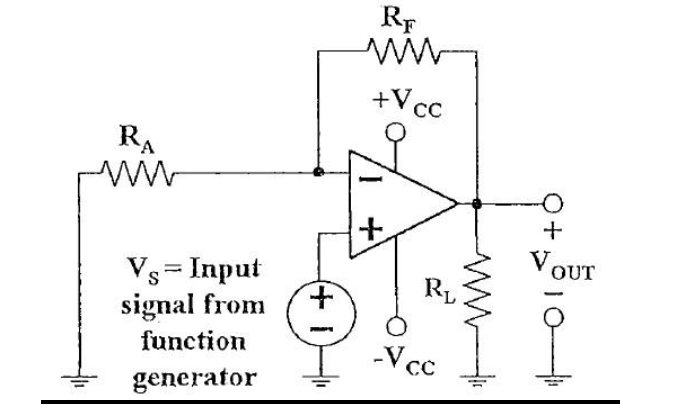
\includegraphics[scale=1]{noninverting.png}
\caption{Non-inverting amplifier.}\label{FigNonInv}
\end{figure}

For non-inverting amplifier, the theoretical gain should be:
$$Gain = \frac{V_{output}}{V_S} = 1 + \frac{R_F}{R_A}$$

\subsubsection{Function generator}

\begin{figure}[H]
\centering
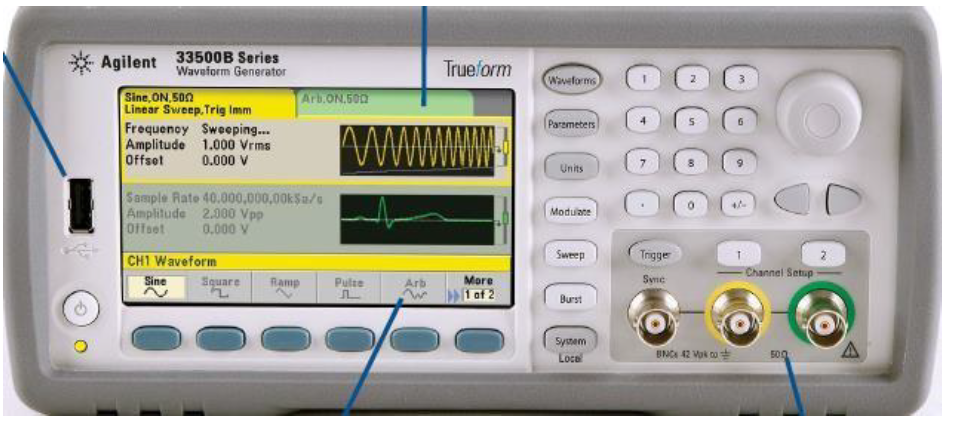
\includegraphics[scale=0.8]{function.png}
\caption{Function generator.}\label{FigFunction}
\end{figure}
Note: the amplitude here equals to half of the pp value (i.e. If you set a wave whose amplitude is 100mV, the measured pp value would be 200 $\text{V}_{\text{pp}}$ where the subscript pp means peak to peak value). 

\subsubsection{Oscilloscope}

\begin{figure}[H]
\centering
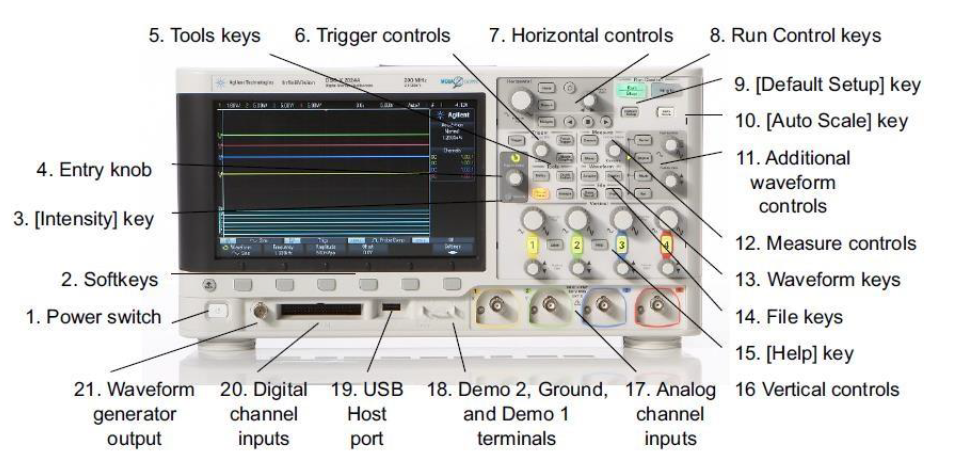
\includegraphics[scale=1.0]{oscilloscope.png}
\caption{Oscilloscope.png}\label{FigOs}
\end{figure}

\begin{enumerate}
\item “Auto scale”: to automatically achieve an output on the screen with proper scale
\item “Meas”: to turn on the measurement of the wave
\item “1”/”2”: to show or hide the wave you detecting through channel 1 or 2
\end{enumerate}



		\section{Results and Discussion}
		
	\subsection{Non-inverting amplifier}

The results of the non-inverting amplifier experiment are shown in Table \ref{TableO1} and Table \ref{TableV1}.

\begin{table}[H]
\centering
\begin{tabular}{lr}
\toprule
$R_1[\Omega]$ & 50.3\\
$R_f[\Omega]$ & 99.6\\
\midrule
$+V_{CC}[V]$ & 5.01\\
$-V_{CC}[V]$ & -5.01\\
\bottomrule
\end{tabular}
\caption{Measurement result of resistances and voltage supply.}\label{TableO1}
\end{table}

\begin{table}[H]
\centering
\begin{tabular}{ccc}
\toprule
$V_{pp(in)}[\text{V}]$ & $V_{pp(out)}[\text{V}]$ & ${V_{pp(out)}}/{V_{pp(in)}}$\\
\midrule
0.100 & 0.312 & 3.12\\
0.200 & 0.600 & 3.00\\
0.300 & 0.848 & 2.83\\
0.400 & 1.34 & 3.35\\
0.500 & 1.60 & 3.20\\
0.600 & 1.92 & 3.20\\
0.700 & 2.18 & 3.11\\
0.800 & 2.50 & 3.13\\
0.900 & 2.86 & 3.18\\
1.000 & 3.14 & 3.14\\
\bottomrule
\end{tabular}
\caption{The input-output voltage relationship.}\label{TableV1}
\end{table}

From figure \ref{FigNonFit} we can see that, $V_{pp(out)}$ vs. $V_{pp(in)}$ assumes linear relationship and the slope indicates the gain of the op amp is about 3.17. The theoretical gain is 
$$Gain = 1 + \frac{R_f}{R_1} = 1 + \frac{99.6}{50.3} = 2.98.$$
The relative error is 
$$\epsilon_{Gain} = \frac{3.17-2.98}{2.91}\times 100\% =6.38\,\%.$$
Our result agrees with the theoretical value.

\begin{figure}[H]
\centering
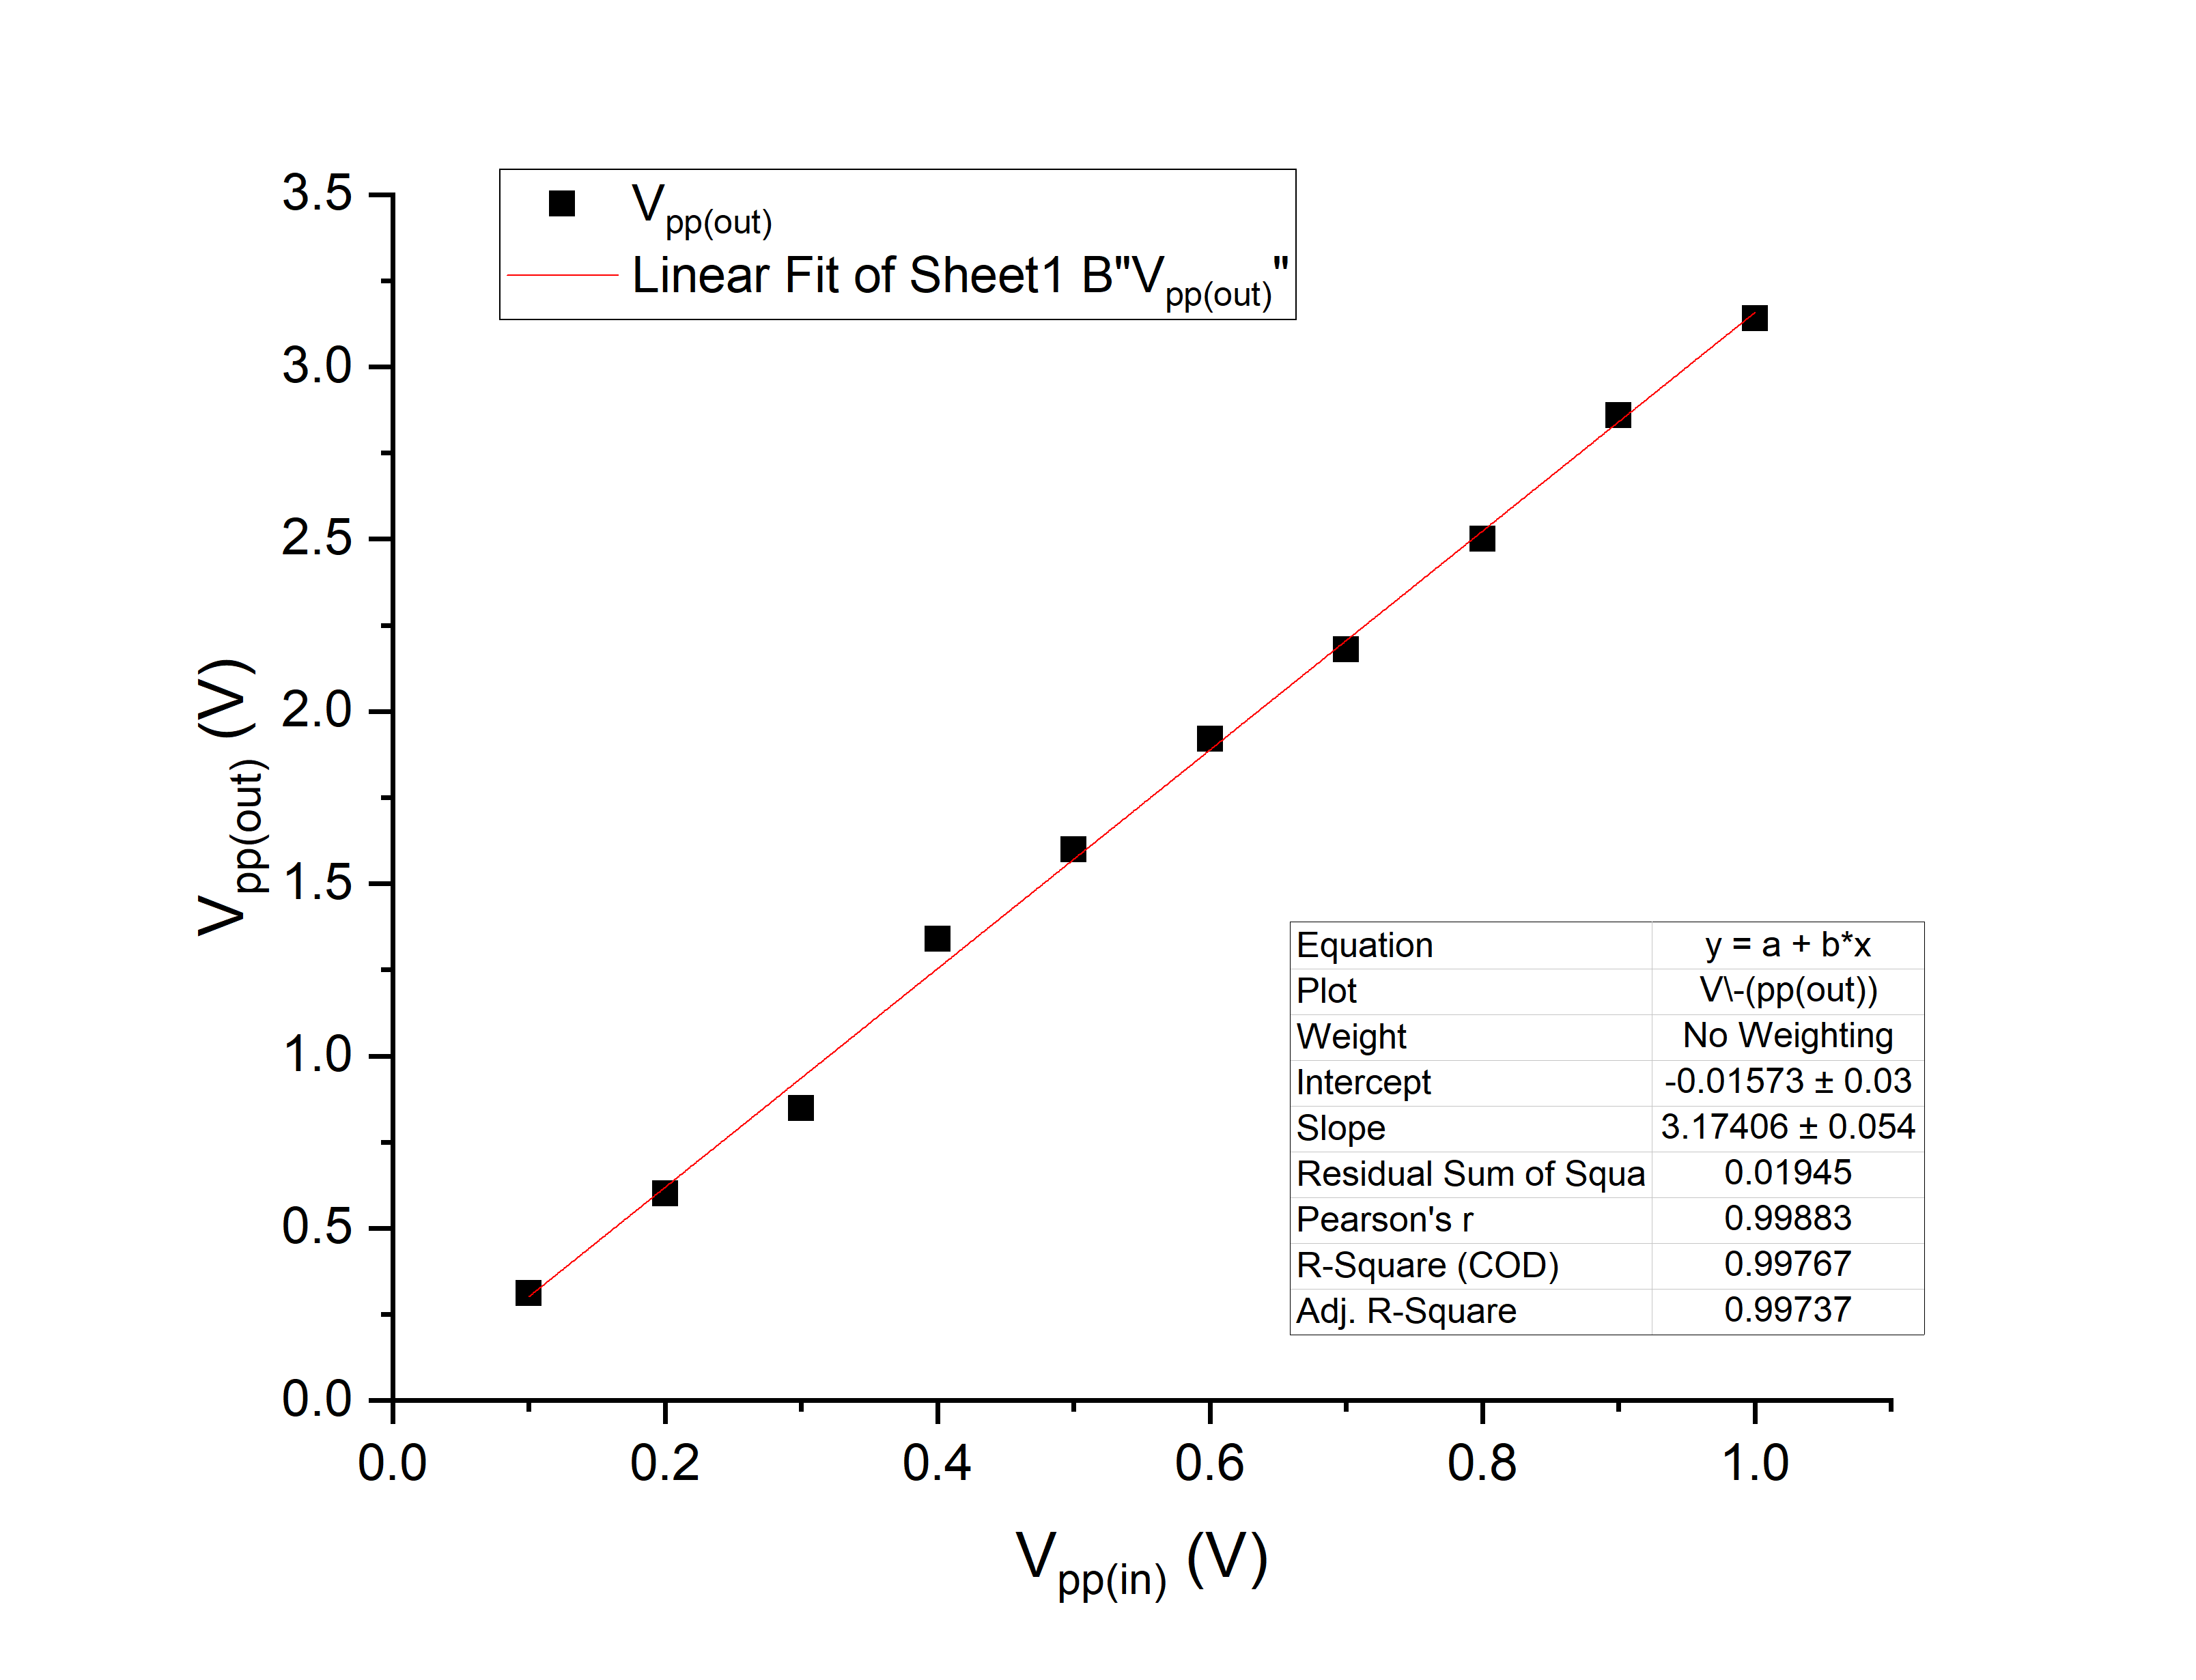
\includegraphics[scale=0.4]{plot1.png}
\caption{Linear fit of $V_{pp(out)}$ vs. $V_{pp(in)}$ relation.}\label{FigNonFit}
\end{figure}

\begin{figure}[H]
\centering
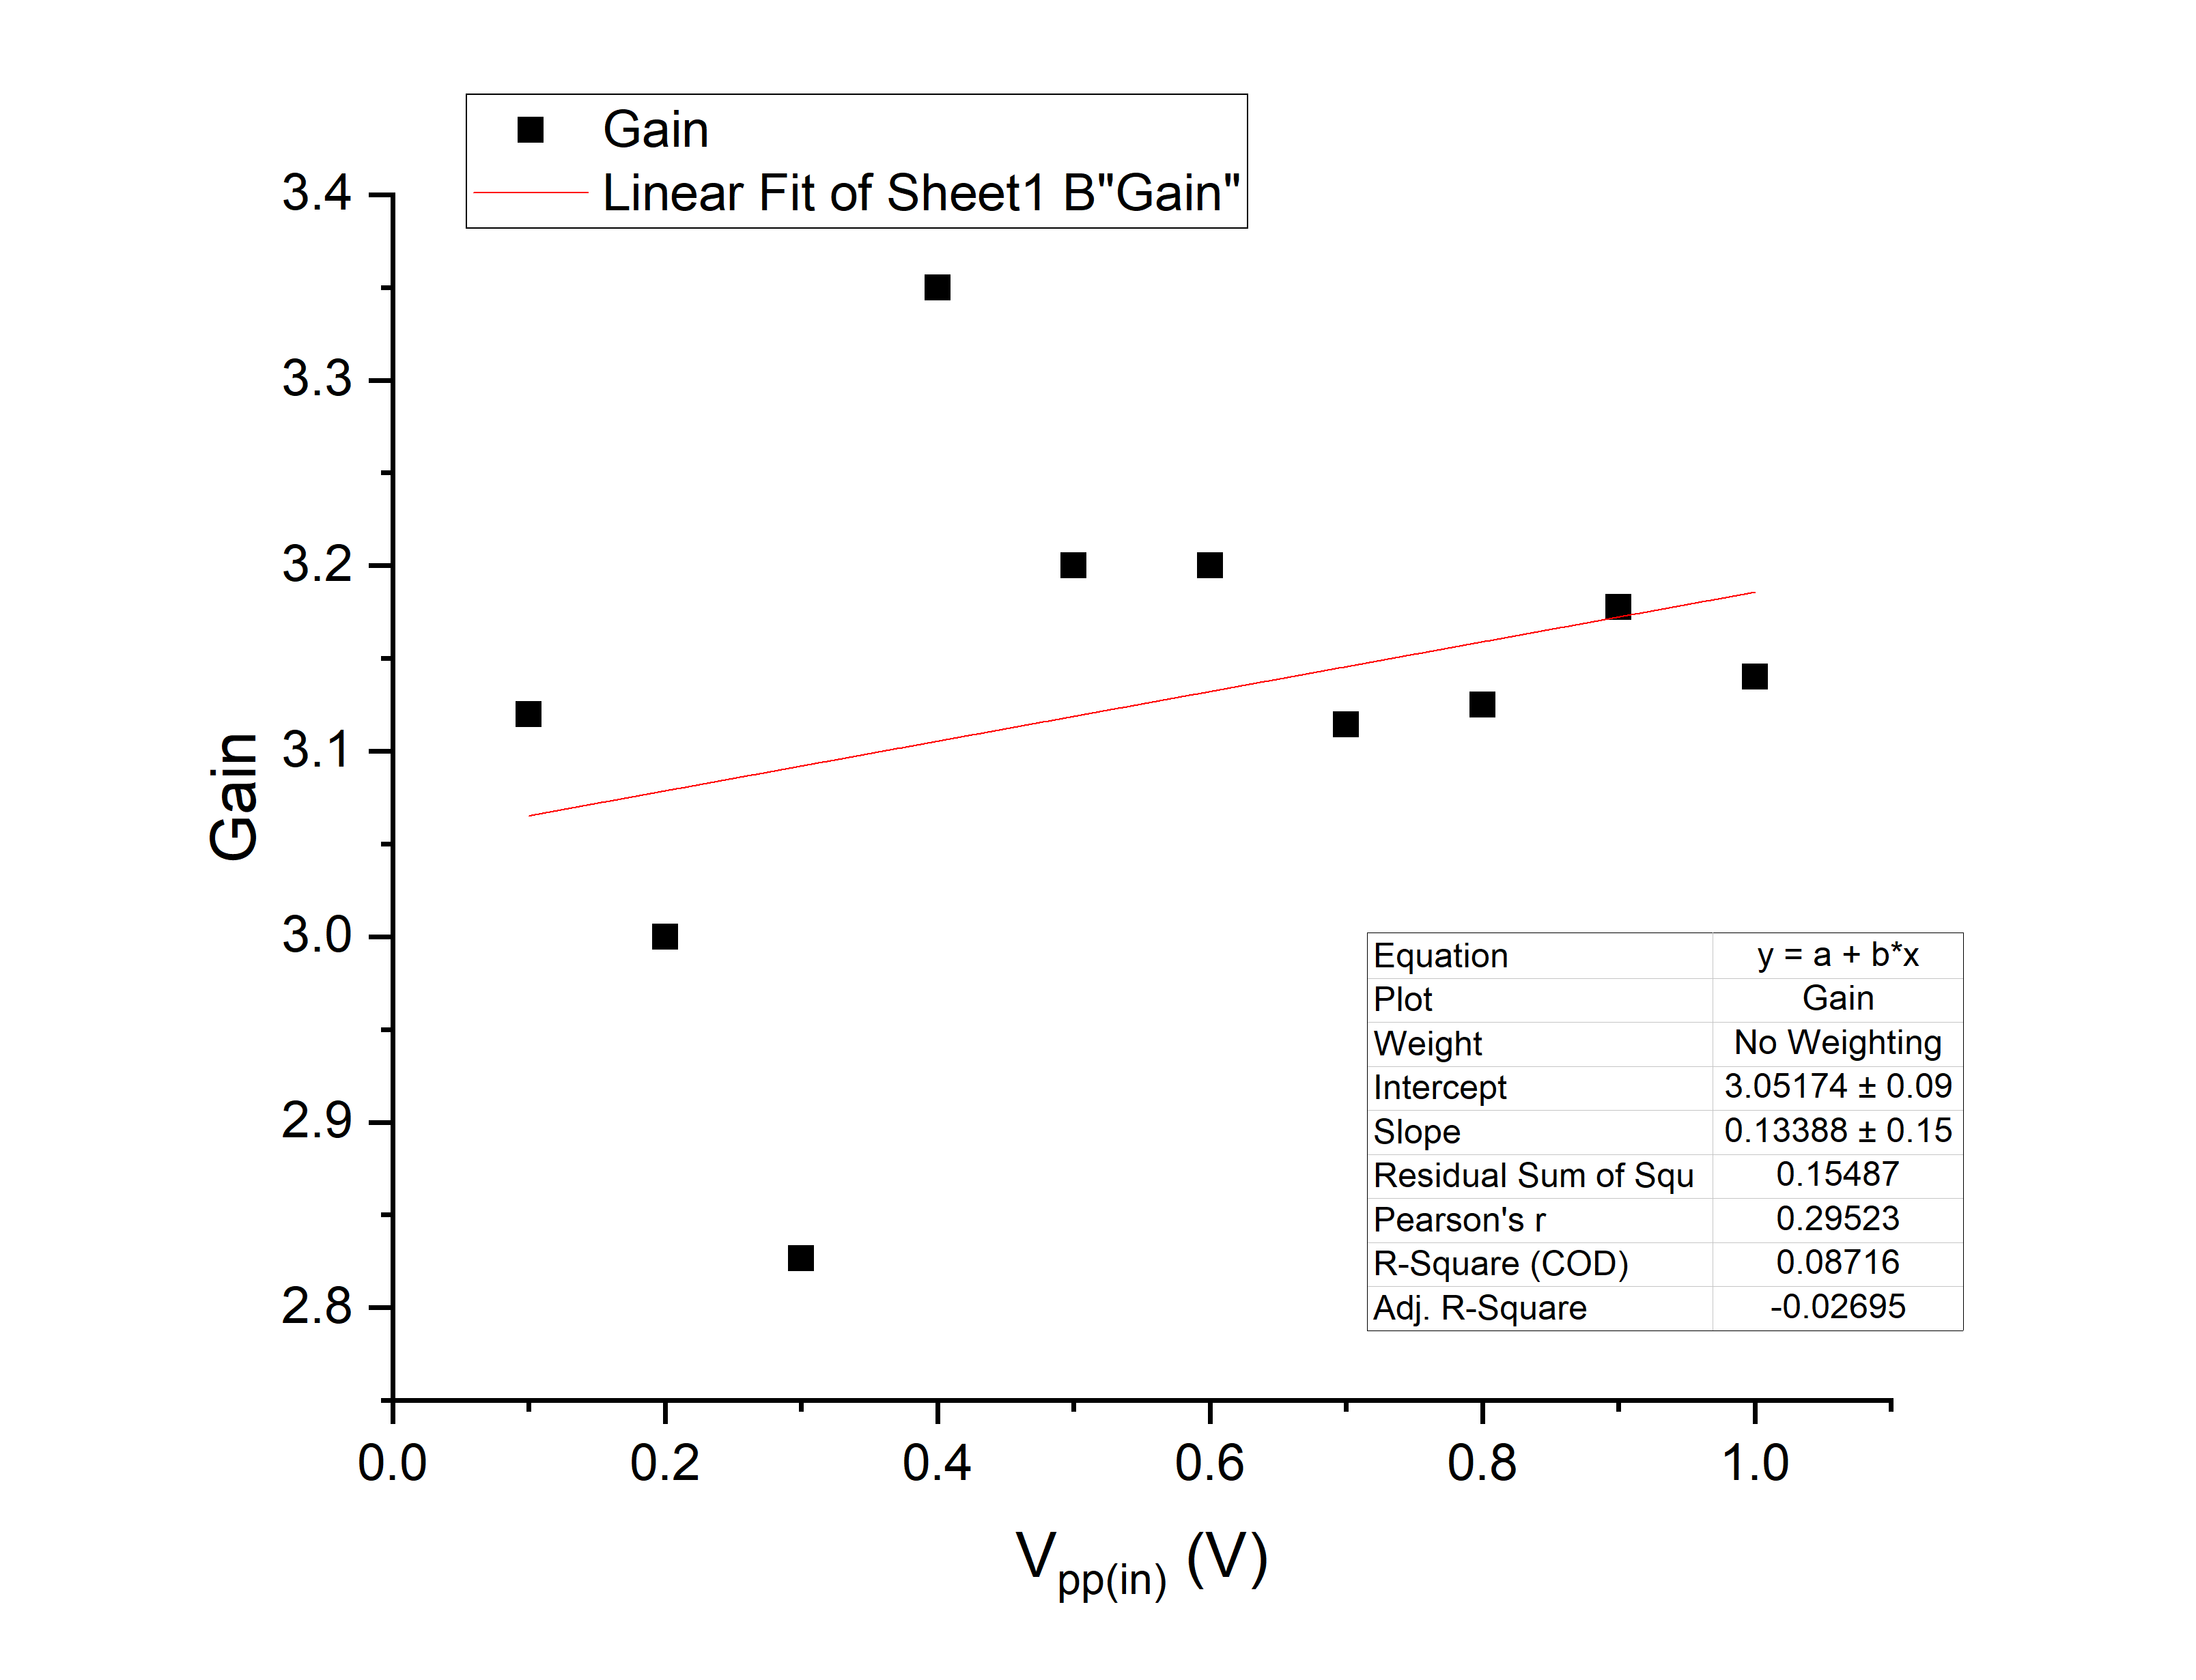
\includegraphics[scale=0.4]{plot2.png}
\caption{Gain vs. $V_{pp(in)}$ relation.}\label{FigG1}
\end{figure}

Figure \ref{FigG1} shows that the gain is independent of the input voltage, since the slope is 0.13 and the Pearson's relative coefficient is much smaller than 1.


	\subsection{Inverting amplifier}

The results of the inverting amplifier experiment are shown in Table \ref{TableO2} and Table \ref{TableV2}.

\begin{table}[H]
\centering
\begin{tabular}{lr}
\toprule
$R_1[\Omega]$ & 50.3\\
$R_f[\Omega]$ & 99.6\\
\midrule
$+V_{CC}[V]$ & 5.01\\
$-V_{CC}[V]$ & -5.01\\
\bottomrule
\end{tabular}
\caption{Measurement results of resistances and voltage supply.}\label{TableO2}
\end{table}

\begin{table}[H]
\centering
\begin{tabular}{ccc}
\toprule
$V_{pp(in)}[\text{V}]$ & $V_{pp(out)}[\text{V}]$ & $V_{pp(out)}/V_{pp(in)}$\\
\midrule
0.1 & -0.116 & -1.16\\
0.2 & -0.224 & -1.12\\
0.3 & -0.312 & -1.04\\
0.4 & -0.396 & -0.99\\
0.5 & -0.433 & -0.87\\
0.6 & -0.592 & -0.97\\
0.7 & -0.688 & -0.98\\
0.8 & -0.792 & -0.99\\
0.9 & -0.896 & -1.00\\
1.0 & -0.984 & -0.98\\
\bottomrule
\end{tabular}
\caption{The input-output voltage relationship.}\label{TableV2}
\end{table}


From figure \ref{FigInvFit} we can see that, $V_{pp(out)}$ vs. $V_{pp(in)}$ assumes linear relationship and the slope indicates the gain of the op amp is about -0.97. However, the theoretical gain is 
$$Gain = -\frac{R_f}{R_1} = -\frac{99.6}{50.3} = -1.98.$$
The relative error is 
$$\epsilon_{Gain} = \frac{-1.98-(-0.97)}{(-1/98)}\times 100\% =51.0\,\%.$$
We have checked our experimental circuit for many times and are sure that the circuit is out of problem. However, our experiment fails to produce the satisfying results. The gain we obtained is only half of the theoretical gain. After thinking about that, we think that it may due to the internal resistance of the function generator. In the non-inverting op amp circuit, the internal resistance of the function generator is connected in parallel, while in the inverting circuit, the internal resistance is connected in series in the circuit. Moreover, the op amp circuit in our experiment is not ideal. This may result in a significant error of our experiment.

\begin{figure}[H]
\centering
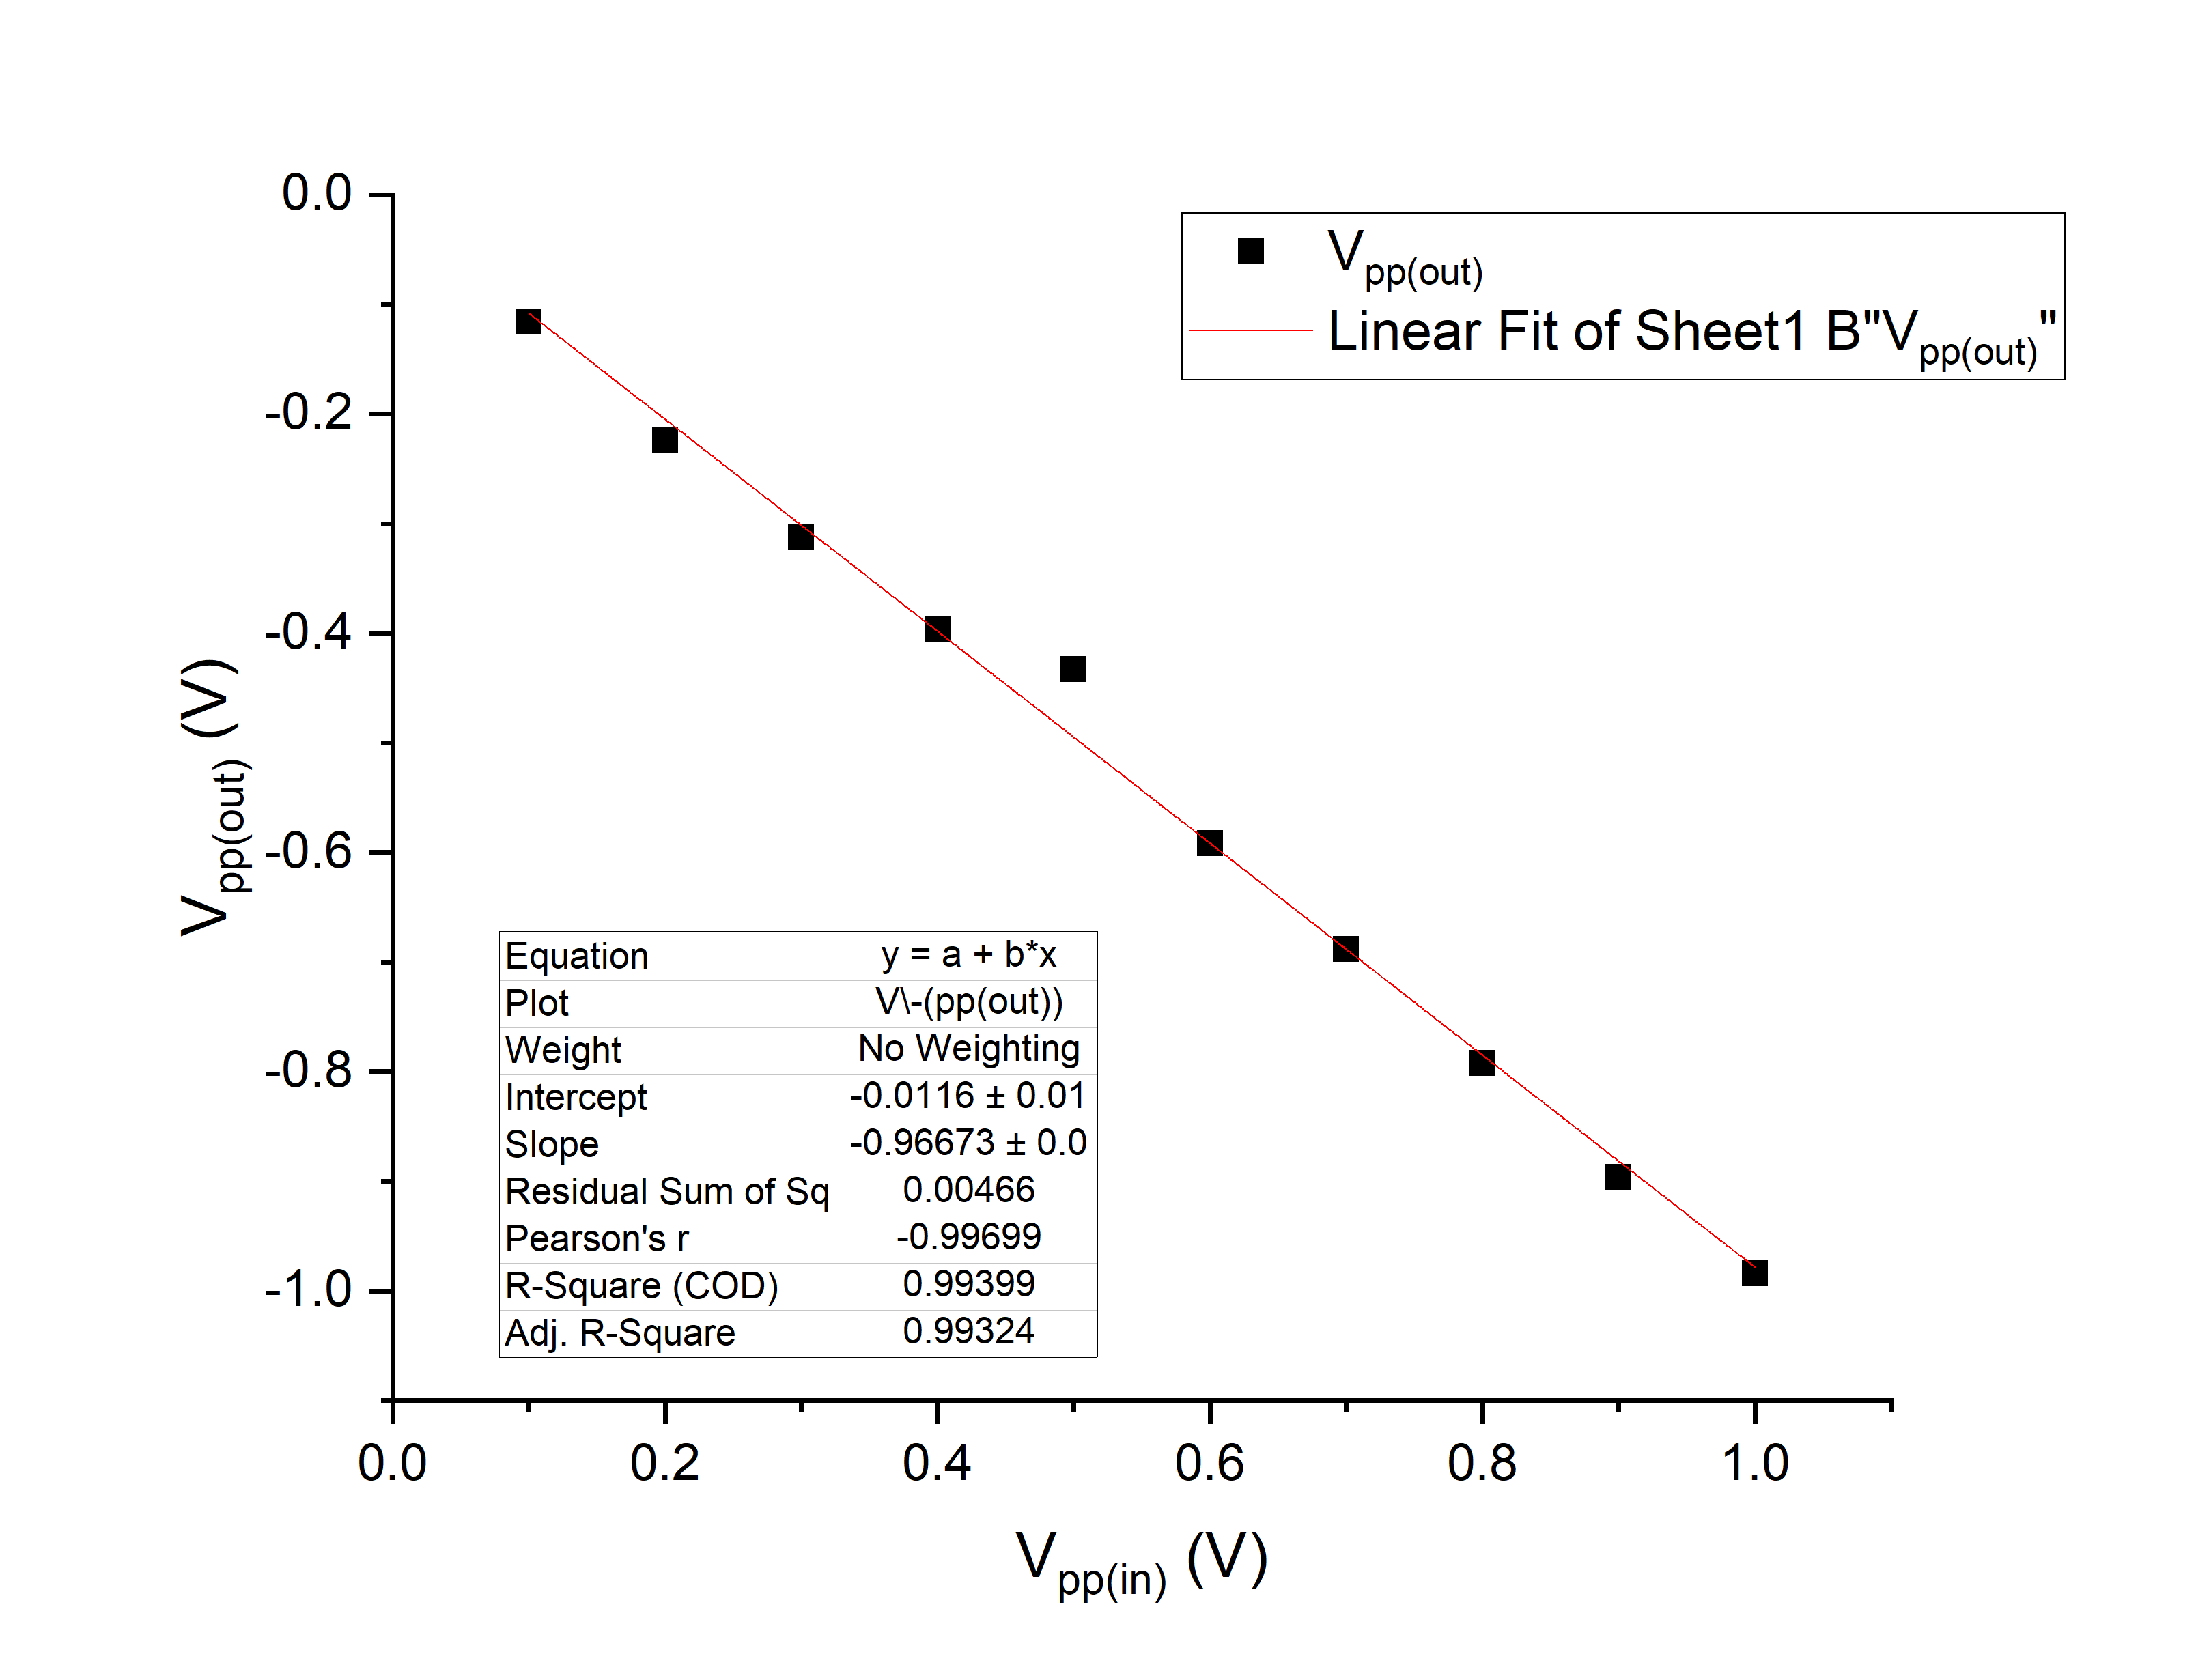
\includegraphics[scale=0.35]{plot3.png}
\caption{Linear fit of $V_{pp(out)}$ vs. $V_{pp(in)}$ relation.}\label{FigInvFit}
\end{figure}

\begin{figure}[H]
\centering
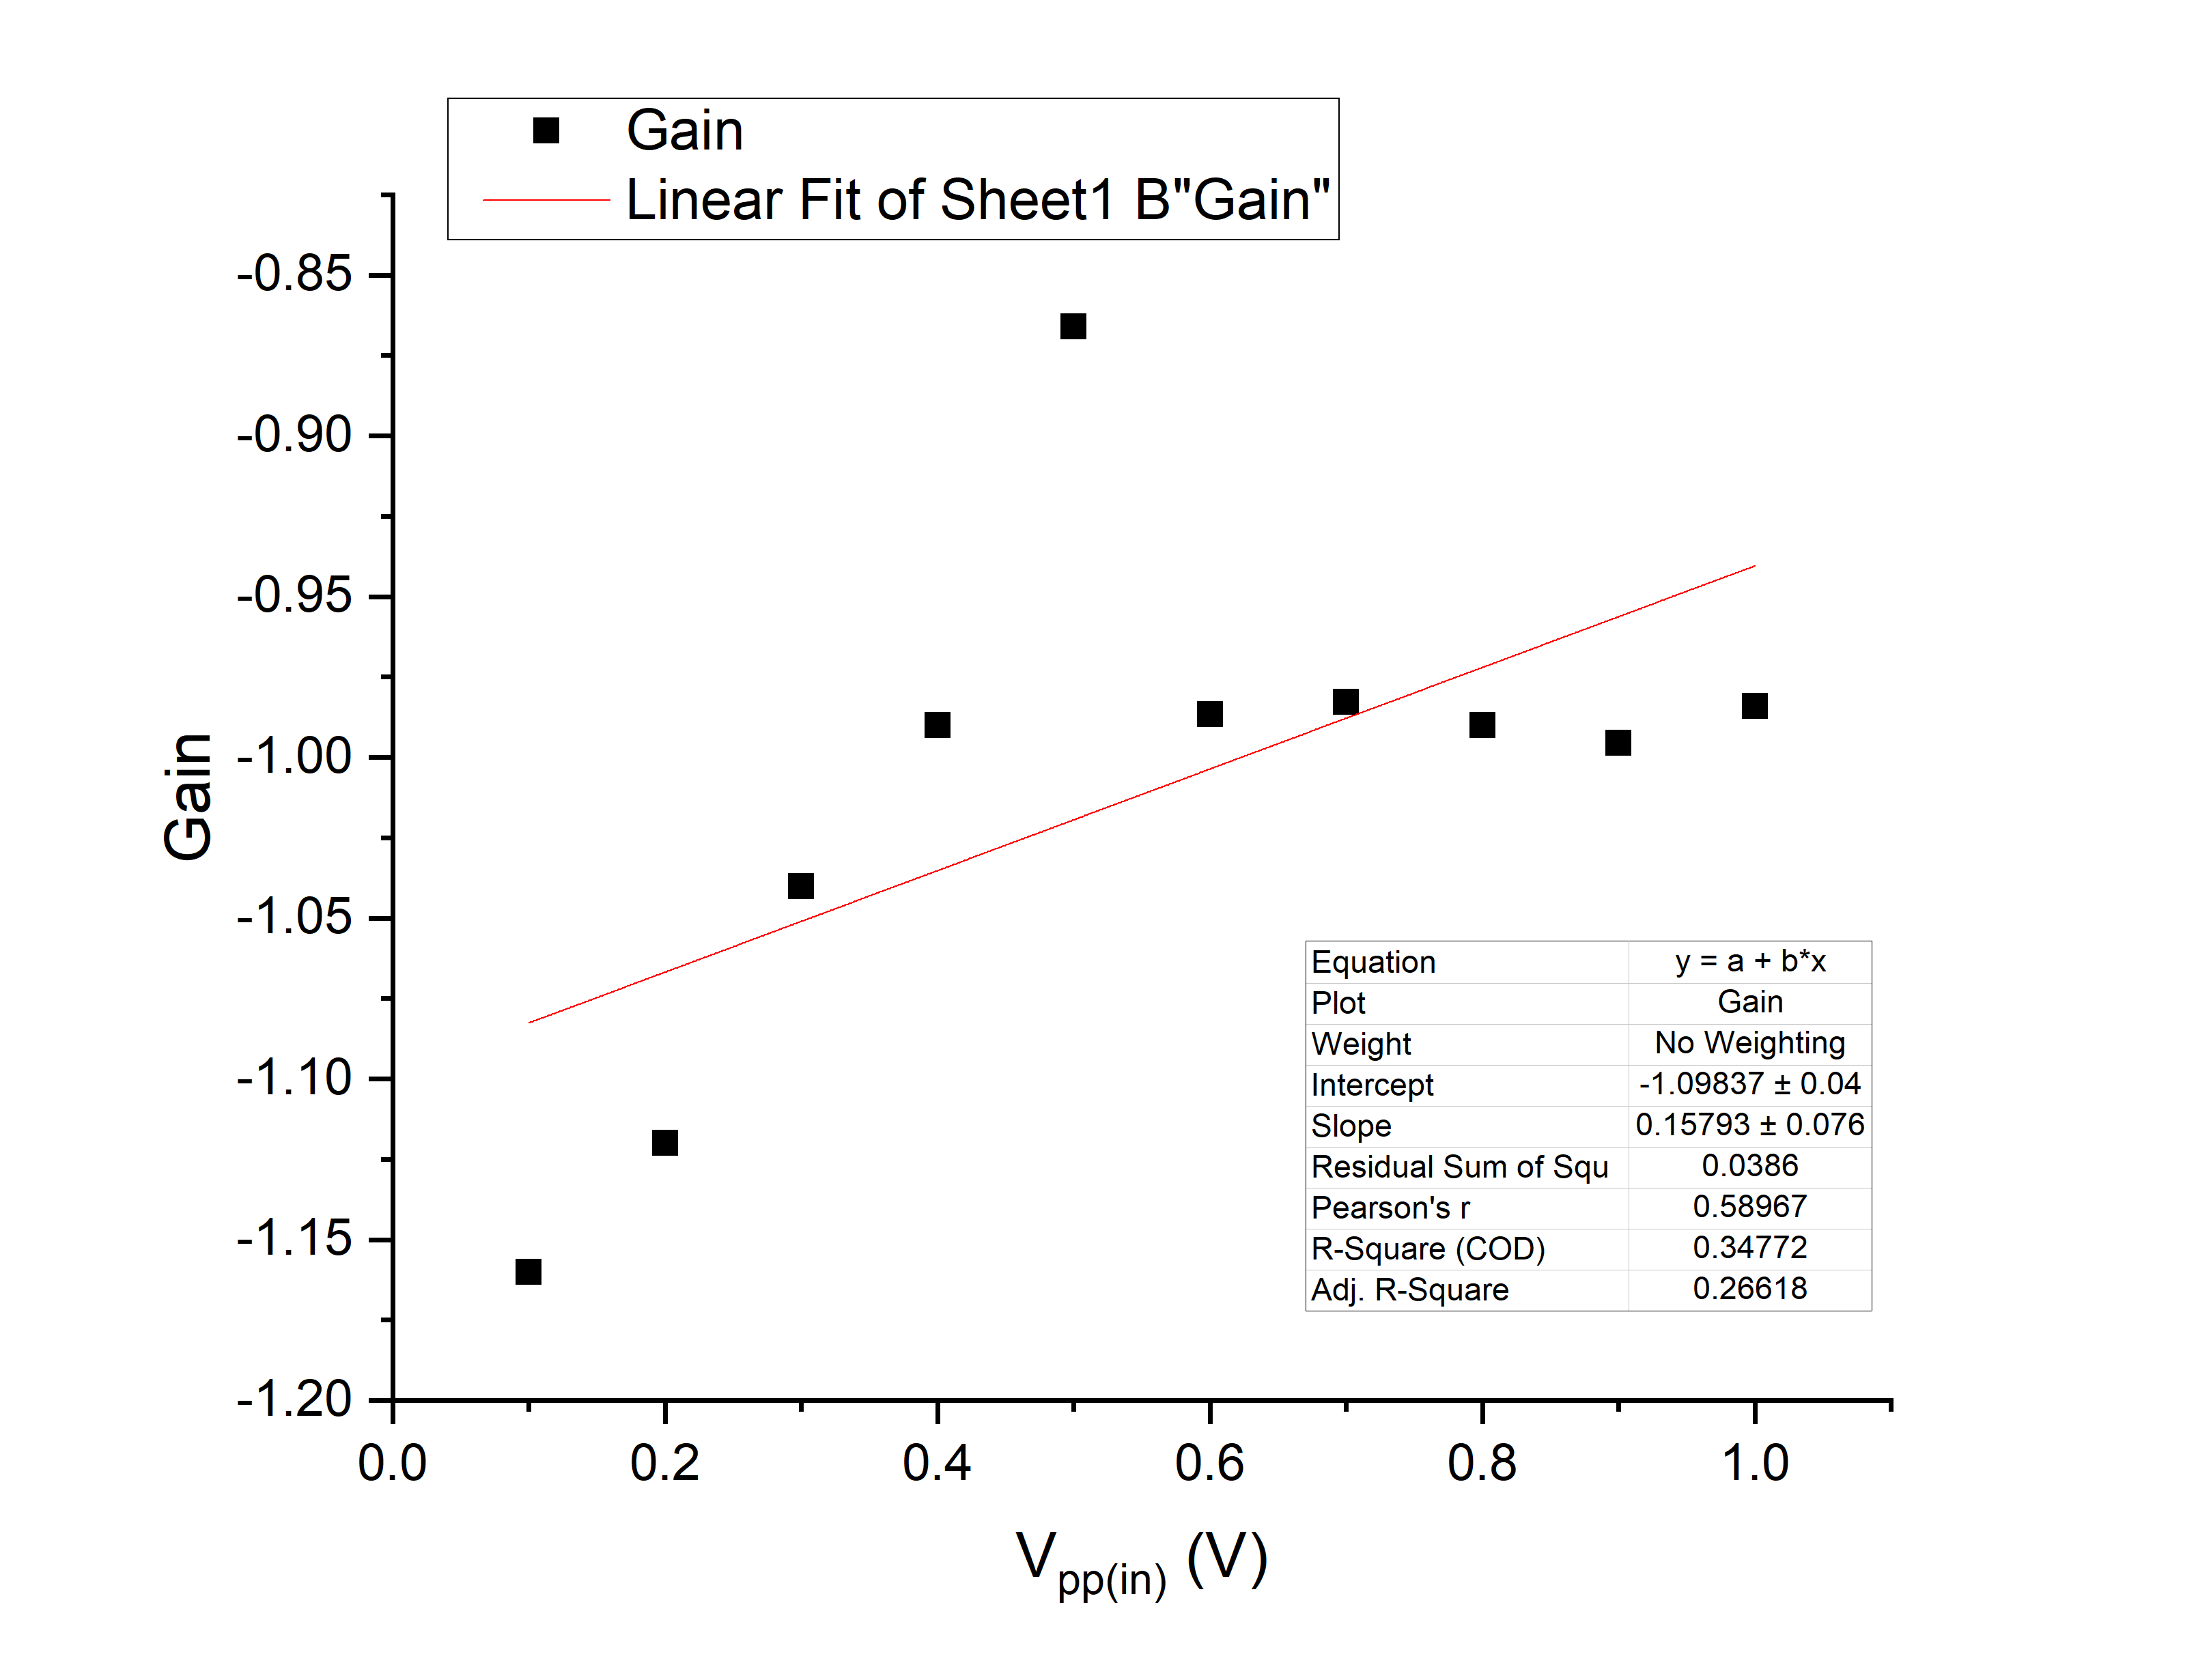
\includegraphics[scale=0.35]{plot4.png}
\caption{Gain vs. $V_{pp(in)}$ relation.}\label{FigG2}
\end{figure}

Figure \ref{FigG1} shows that the gain is independent of the input voltage, since the slope is 0.16 and the Pearson's relative coefficient is much smaller than 1.

\section{Conclusion}
In this lab, we verify that the non-inverting and inverting op amp. The gain of the non-inverting amplifier is $Gain = 1+\frac{R_F}{R_A},$
and the gain of the inverting amplifier is $Gain = -\frac{R_F}{R_A}.$
We also learn how to use a function generator and how to operate on the oscillator.

\section{References}
\noindent [1] VE215 Lab2 Manual

\section{Appendix}
The data sheet is attached at the end of the report.

\end{document}
